% Evolution and Unified Performance Evaluation of Clustering Techniques
% in Heterogeneous Wireless Sensor Networks
%
% Build:  pdflatex main && bibtex main && pdflatex main && pdflatex main
%
% House rules for this manuscript (see docs/PAPER_REVISION_NOTES.md):
%   * No em dashes anywhere. Use commas, colons, semicolons or parentheses.
%   * Every number in the prose is traceable to a CSV under results/.
%   * Tables are generated by scripts/make_tables.py and are not hand-edited.

\documentclass[conference]{IEEEtran}

\usepackage{amsmath,amssymb}
\usepackage{booktabs}
\usepackage{graphicx}
\usepackage{url}
\usepackage[hidelinks]{hyperref}

\graphicspath{{../results/analysis/figures_paper/}{../results/analysis/figures_lossy/}}

\begin{document}

\title{Evolution and Unified Performance Evaluation of\\
Clustering Techniques in Heterogeneous\\
Wireless Sensor Networks}

\author{%
\IEEEauthorblockN{Ashish Sharma, Yogesh Sharma}
\IEEEauthorblockA{Assistant Professor, Department of Computer Science and Engineering\\
Maharaja Agrasen Institute of Technology, Delhi, India\\
ashish@mait.ac.in, yogeshsharma@mait.ac.in}
\and
\IEEEauthorblockN{Vansh Tomar, Satvik Rastogi, Ansh Rai}
\IEEEauthorblockA{Department of Computer Science and Engineering\\
Maharaja Agrasen Institute of Technology, Delhi, India\\
vanshwar@gmail.com, satvikrastogi777@gmail.com, raiansh230405@gmail.com}
}

\maketitle

\begin{abstract}
Wireless sensor nodes spend most of their energy on the radio and rarely get a
new battery, so lifetime is decided by how the network organizes its
transmissions. Clustering is the standard answer, and twenty-five years of
clustering protocols now span three methodological generations: probabilistic
and threshold heuristics, explicit optimization, and learned selection
functions. Those generations are usually compared by reading their published
tables side by side, which does not work, because each protocol was measured
against a different simulator, field size, node count, energy budget and
channel. We rebuild the comparison from scratch. Nine protocols spanning all
three generations, plus a direct-transmission baseline, run on a single engine
that owns energy accounting, packet sizing, fusion, the channel and the
counting of delivered readings; a protocol returns only a cluster structure, and
a static audit confirms that no implementation touches the energy or liveness
arrays. Trials are paired, so at a given index every protocol sees the same
topology, the same per-link shadowing and the same sensed-value stream, and the
resulting differences are tested with sign-flip permutation, paired bootstrap
intervals and Holm correction. Running the whole study at both endpoints of the
one parameter the source specifications leave open, transmit power, retracts one
of our own comparisons: the first-death advantage of the type-2 fuzzy protocol
and the deep Q-network over LEACH is 417 and 426 rounds under packet loss and
falls to 17 and 22 rounds, no longer significant, once loss is removed. Their
advantage in overall survival and in readings delivered survives both channels.
A 1{,}350-run sweep over three node counts and three field areas shows the same
boundary from the other side: distance to the sink, not node density, sets the
regime, and in a $50\times50$~m field clustering is worse than no clustering at
all. We report the mechanism by measurement rather than by argument, and we
disclose the modeling choices that bound the results, ordered by how far each
could move a conclusion.
\end{abstract}

\begin{IEEEkeywords}
Wireless sensor networks, clustering protocols, network lifetime, energy
efficiency, reinforcement learning, graph neural networks, type-2 fuzzy logic,
cluster head selection, reproducibility.
\end{IEEEkeywords}

\section{Introduction}
\label{sec:intro}

A wireless sensor node spends most of its energy on its radio, and in nearly all
deployments its battery cannot be replaced~\cite{akyildiz2002survey}. Lifetime
is therefore decided by how the network organizes its transmissions rather than
by any property of the sensing hardware. Clustering is the standard response:
nodes elect a subset of themselves as cluster heads, members send short-range
packets to their head, and the head fuses them into one packet and pays the
single expensive transmission to the base station. Because that role is
expensive it has to rotate, and the question every clustering protocol answers
is which nodes should carry it this round.

Twenty-five years of answers fall into three broad generations. The first is
heuristic. LEACH rotates the role by an independent probabilistic threshold with
an epoch constraint~\cite{heinzelman2000leach}; PEGASIS abandons clusters
entirely for a greedy chain in which each node talks only to its nearest
neighbor~\cite{lindsey2002pegasis}; TEEN and its extension APTEEN leave the
topology alone and instead suppress transmissions that fall below a sensed-value
threshold~\cite{manjeshwar2001teen,manjeshwar2002apteen}. Later heuristics
such as HEED refine the election rule without changing its
character~\cite{younis2004heed,abbasi2007clustering}. The second generation
replaces the heuristic with an explicit objective. Head selection is posed as a
multi-objective optimization problem and solved with
NSGA-II~\cite{deb2002nsga2}, or encoded in a type-2 fuzzy rule base that reasons
over residual energy, distance and local density under linguistic
uncertainty~\cite{mendel2002type2,karnik2001centroid}. The third generation
learns the selection function instead of specifying
it~\cite{alsheikh2014ml}: a self-organizing map places heads by
unsupervised vector quantization~\cite{kohonen1990som}, a deep Q-network treats
rotation as a sequential decision problem~\cite{mnih2015dqn,sutton2018rl}, and
a graph convolutional network scores candidates from the topology's adjacency
structure~\cite{kipf2017gcn,wu2021gnnsurvey}.

The generations are usually compared by reading their published tables side by
side, and that comparison does not hold. Each protocol was proposed against a
different simulator, field size, node count, packet length and energy
budget~\cite{kurkowski2005incredibles,pawlikowski2002credibility,andel2006credibility},
almost always
against LEACH alone, and almost always on a lossless channel. More
consequentially, the assumptions that decide the outcome are rarely stated.
Whether a centralized protocol is charged for the uplink that tells the base
station each node's residual energy can be worth a quarter of the entire energy
budget over a long run. Whether fusion is lossless in bits determines how much a
chain protocol gains over a clustered one. Whether lifetime is reported at first
death, half death or last death can reverse a ranking outright, and the author
chooses which to report. A margin obtained under one set of these choices is not
evidence about the algorithm; it is partly evidence about the harness.

This paper measures the three generations in one harness. Nine protocols
spanning all of them, plus a direct-transmission baseline, run on a single
engine over 30 paired trials in each of two channel configurations, for 600 runs
in the headline study, and over a further 1{,}350 runs in a node-count by
field-area sweep. Run index $i$ seeds the topology, the per-link shadowing and
the entire sensed-value stream identically for every protocol, so a comparison
at a given index is genuinely paired rather than an average over unrelated
worlds. Fairness is enforced structurally instead of by convention: the engine
owns energy accounting through a single charging function, packet sizing, the
aggregation charge, the channel and its ARQ retries, and the counting of
delivered readings. A protocol returns only a cluster structure and a route
shape, and a static audit verifies that no protocol implementation writes to the
energy or liveness arrays. Every protocol runs on the same numerical substrate,
hand-written NumPy including the backpropagation for both learned models,
because per-round setup time is a reported metric and mixing frameworks would
corrupt it. No protocol is tuned to reproduce any published number;
disagreement with the source tables is expected and is not treated as error.

We also state up front the one assumption that most favors part of the field.
Centralized protocols are not charged for the uplink that carries node state to
the sink, because that state is treated as piggybacked on data traffic the
network already sends. This is the standard convention in the centralized
clustering literature, but it is still a choice, and Section~\ref{sec:validity}
measures what it is worth: LEACH spends 12.73\% of its consumed energy on
control traffic against 2.33\% to 3.95\% for the centralized five, so every
comparison that crosses those classes carries a subsidy of roughly nine to ten
percentage points of the budget.

Five results are worth stating before the details.

Transmit power is not a background parameter but a determinant of the ranking.
Repeating the entire study on a lossless channel removes the first-death
advantage of the type-2 fuzzy protocol and of the DQN over LEACH altogether:
$+417$ and $+426$ rounds at $p_{\mathrm{Holm}} = 0.00045$ under packet loss,
falling to $+17$ and $+22$ rounds and no significance once loss is removed.

Direct measurement of where the energy goes explains why, and the explanation is
not the obvious one. Packet error is effectively zero below 120~m, and every
protocol's \emph{mean} head-to-sink distance sits below that, so the mean cannot
be the cause. The tail can. LEACH puts 29.9\% of its head-rounds beyond 120~m
and spends 6.39\% of its budget on retransmissions; the DQN puts 5.1\% of its
head-rounds out there and spends 2.31\%. Across the six single-hop protocols the
share of head-rounds beyond 120~m predicts retry energy share with $r = 0.95$.
What the newer protocols demonstrably do well is keep the far tail of the
head-to-sink hop out of the error waterfall, and that skill pays only in
proportion to how lossy the hop is.

The effect is specific to first death. Differences in area under the alive-node
curve and in readings delivered hold at $p_{\mathrm{Holm}} = 0.00045$ in both
channels.

No single lifetime figure summarizes clustering, because it buys a later first
death by bringing the last death forward. LEACH reaches first death at 1{,}046
rounds against the baseline's 114, a factor of 9.2, while dying out completely
at 2{,}191 rounds against the baseline's 3{,}202. The GCN is the extreme case,
with a first death 3.1 times earlier than LEACH's and a last death 45\% later.

Finally, the advantage of clustering is a property of an operating regime rather
than of clustering as such. Across a $3\times3$ grid of node counts and field
areas, tripling the node count moves first death by a factor of 0.88 to 1.26
while tripling the field side moves it by a factor of 5 to 7. In the
$50\times50$~m field, where no link reaches the error waterfall, LEACH is
outlived by the no-clustering baseline.

The reactive protocols sit outside all of this because they survive by not
reporting: TEEN and APTEEN fail to reach last death within the 7{,}000-round cap
in all 30 trials, at a data yield of 0.11 and 0.12 against roughly 0.9 for the
proactive protocols.

The contributions are as follows. First, a single simulation engine in which
nine clustering protocols from three methodological generations execute under
provably identical physical conditions, with fairness enforced by construction
rather than by author discipline. Second, a paired experimental design, common
topology, shadowing and sensed-data stream per trial index, analyzed with paired
sign-flip permutation tests, paired bootstrap intervals and Holm correction
across the protocol family, in place of the unpaired mean-and-deviation
comparison the literature normally reports. Third, a channel sensitivity pair
run as a rule rather than as an appendix: a conclusion that survives both the
lossy and the ideal configuration is a statement about the protocol, and one
that flips is a statement about transmit power. Applying the rule retracts a
comparison that the lossy channel alone would have supported. Fourth, a
node-count by field-area sweep that identifies the regime boundary from an
independent direction and tests whether the frozen learned policies transfer off
their training distribution. Fifth, mechanistic explanations obtained by
measurement rather than argument, including the energy split by category, the
distribution of cluster-head distance relative to the radio crossover, and
cluster-head rotation concentration. Sixth, a full disclosure of the modeling
choices that bound these results, ordered by how far each could move a
conclusion, together with the reproduction artifacts.

Section~\ref{sec:model} describes the system and radio model,
Section~\ref{sec:protocols} the nine protocols and their fairness-relevant
implementation details, Section~\ref{sec:design} the experimental design and
statistical procedure, Section~\ref{sec:results} the results,
Section~\ref{sec:validity} the threats to validity, and
Section~\ref{sec:conclusion} concludes.

\section{System Model}
\label{sec:model}

\begin{table}[!t]
\caption{Simulation parameters. Every value is read from the single frozen configuration object used by all ten protocols; nothing is protocol-specific.}
\label{tab:parameters}
\centering
\begin{tabular}{ll}
\toprule
Parameter & Value \\
\midrule
\multicolumn{2}{l}{\textit{Topology and energy}} \\
\quad Nodes $N$ & 100 \\
\quad Field & 100 $\times$ 100 m \\
\quad Base station & $(50, 150)$ m \\
\quad Initial energy $E_0$ & 1.0 J per node \\
\quad Rounds (cap) & 7,000 \\
\quad Runs per configuration & 30 \\
\addlinespace
\multicolumn{2}{l}{\textit{Packets}} \\
\quad Data packet & 4,000 bits \\
\quad Control packet & 200 bits \\
\addlinespace
\multicolumn{2}{l}{\textit{Radio (first-order model)}} \\
\quad $E_{\mathrm{elec}}$ & 50 nJ/bit \\
\quad $\varepsilon_{\mathrm{fs}}$ & 10 pJ/bit/m$^2$ \\
\quad $\varepsilon_{\mathrm{mp}}$ & 0.0013 pJ/bit/m$^4$ \\
\quad $E_{\mathrm{DA}}$ (fusion) & 5 nJ/bit \\
\quad Crossover $d_0$ & 87.7 m \\
\addlinespace
\multicolumn{2}{l}{\textit{Channel}} \\
\quad Transmit power $P_t$ & 12 dBm \\
\quad Path loss at 1 m & 40 dB \\
\quad Path-loss exponent $n$ & 3.0 \\
\quad Shadowing $\sigma$ & 4 dB \\
\quad Noise floor & -105 dBm \\
\quad ARQ retransmissions & 2 \\
\addlinespace
\multicolumn{2}{l}{\textit{Sensed data (Ornstein--Uhlenbeck)}} \\
\quad Mean $\mu$, reversion $\theta$ & 50, 0.05 \\
\quad Step $\sigma$ & 2.0 \\
\quad TEEN/APTEEN $H_T$, $S_T$, $T_C$ & 55, 1.0, 50 rounds \\
\addlinespace
\multicolumn{2}{l}{\textit{Protocol-agnostic}} \\
\quad Head fraction $p$ & 0.05 \\
\quad Density radius & 25 m \\
\quad NSGA-II population, generations & 40, 30 \\
\quad Re-clustering interval & 5 rounds \\
\addlinespace
\multicolumn{2}{l}{\textit{Timing}} \\
\quad Bit rate & 250 kbps \\
\quad Slot / guard / processing & 20 / 4 / 1 ms \\
\bottomrule
\end{tabular}
\end{table}


\subsection{Network and Energy}

One hundred nodes are placed uniformly at random in a $100\times100$~m field,
with the base station outside the field at $(50, 150)$, so node-to-sink
distances span 50 to 158~m. Every node begins with $E_0 = 1$~J, is stationary,
and fails only by depletion. The configuration carries fields for two-level and
three-level heterogeneity~\cite{smaragdakis2004sep,qing2006deec}, disabled
throughout, so every result here is for a homogeneous population.
Table~\ref{tab:parameters} lists every parameter; nothing in it is
protocol-specific, and no constant is defined outside the single frozen
configuration object.

A run proceeds in rounds until the last node dies or a cap of 7{,}000 rounds is
reached. Energy is a linear reservoir with a single charging function: a node
asked to spend more than it holds spends what remains, dies, and loses the
packet in flight. Refusing the transmission instead would strand the remainder
and break the conservation identity
\begin{equation}
\sum_i \left( E_0(i) - E_{\mathrm{res}}(i) \right)
= E_{\mathrm{tx}} + E_{\mathrm{rx}} + E_{\mathrm{ctrl}}
+ E_{\mathrm{agg}} + E_{\mathrm{retry}},
\label{eq:conservation}
\end{equation}
asserted at the end of every run to $10^{-9}$~J and the primary correctness
check on the simulator.

\subsection{Radio Energy}

We use the first-order model of Heinzelman et
al.~\cite{heinzelman2000leach,heinzelman2002appspecific}. Transmitting $k$ bits
over distance $d$ costs
\begin{equation}
E_{\mathrm{tx}}(k, d) =
\begin{cases}
k E_{\mathrm{elec}} + k \varepsilon_{\mathrm{fs}} d^{2}, & d < d_0 \\[2pt]
k E_{\mathrm{elec}} + k \varepsilon_{\mathrm{mp}} d^{4}, & d \geq d_0
\end{cases}
\label{eq:radio}
\end{equation}
with $E_{\mathrm{rx}}(k) = k E_{\mathrm{elec}}$ and a fusion charge of
$E_{\mathrm{DA}}$ per bit received. The crossover
$d_0 = \sqrt{\varepsilon_{\mathrm{fs}}/\varepsilon_{\mathrm{mp}}} = 87.7$~m sits
inside the range of node-to-sink distances, which makes head placement relative
to $d_0$ a live variable: a head at 100~m pays the fourth-power branch and one
at 80~m does not. In the seed-0 topology 36 of the 100 nodes fall inside $d_0$,
against an expected 32.7\% over the placement distribution.

The model is minimal and its omissions matter. There is no idle listening, no
sleep-wake transition energy, no radio startup and no processor energy. Idle
listening often dominates real budgets~\cite{ye2002smac,polastre2004bmac}, and
including it would compress the differences between all nine protocols, so this
bounds every energy figure that follows.

\subsection{Channel}
\label{sec:channel}

Packet loss is derived from a link budget rather than assigned as a constant.
Path loss follows a log-distance law with per-link
shadowing~\cite{rappaport2002wireless},
\begin{equation}
PL(d) = PL_{1\mathrm{m}} + 10 n \log_{10} d + X_\sigma,
\qquad X_\sigma \sim \mathcal{N}(0, \sigma^2),
\label{eq:pathloss}
\end{equation}
giving a receive power of $P_t - PL(d)$ and an SNR against a $-105$~dBm noise
floor. Bit errors follow the closed-form non-coherent BFSK
expression~\cite{proakis2008digital}
$\mathrm{BER} = \tfrac{1}{2}e^{-\gamma/2}$, and
$\mathrm{PER} = 1 - (1-\mathrm{BER})^{k}$, evaluated as
$-\mathrm{expm1}\!\left(k \ln(1-\mathrm{BER})\right)$ for numerical stability.

\begin{figure}[!t]
\centering
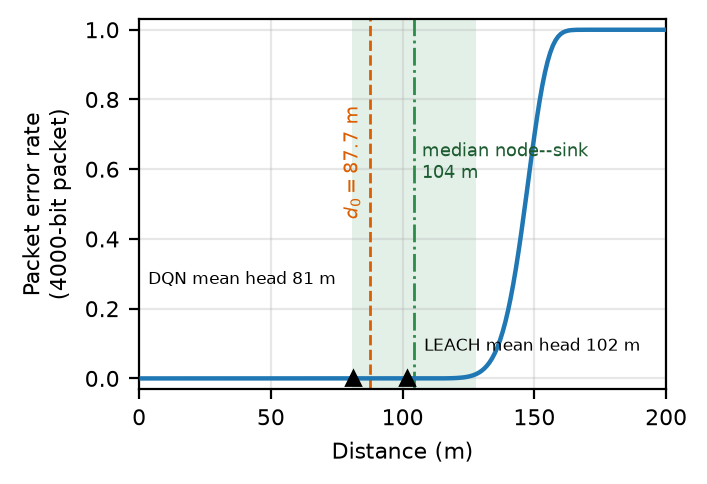
\includegraphics[width=\columnwidth]{figA_per_curve.png}
\caption{Packet error rate against distance for a 4{,}000-bit packet, with the
crossover $d_0 = 87.7$~m and the measured band of node-to-sink distances marked.
The curve is a waterfall, not a gradient: effectively zero out to about 120~m,
saturated by 158~m. Where a protocol places the far tail of its head-to-sink hop
relative to that step decides what it pays in retransmissions, which is why
transmit power is an experimental factor in Section~\ref{sec:design} rather than
a constant.}
\label{fig:per}
\end{figure}

Fig.~\ref{fig:per} plots the result, and it is a waterfall rather than a
gradient. Without shadowing, PER is $2.6\times10^{-8}$ at 100~m,
$1.0\times10^{-3}$ at 120~m, 0.19 at 140~m and 0.97 at 158~m, so the transition
from usable to useless spans about 3.6~dB of SNR and 40~m. Shadowing at
$\sigma = 4$~dB smears that step into a distribution over links and is the
source of the genuine per-topology variance in delivery ratio; it is drawn once
per topology and held fixed, because the nodes are static. Failed packets are
retried up to twice, each attempt paying full transmit and receive energy, which
is what makes a lossy channel cost joules rather than only packets. Retry energy
is charged to a separate category so it can be measured directly rather than
inferred.

\subsection{Control-Traffic Accounting}
\label{sec:control}

Control traffic is charged by the engine according to the protocol's declared
class, not by the protocol itself, and both endpoints pay. Distributed protocols
pay a full handshake every round: an advertisement priced at the distance to the
farthest joiner with a receive charge on every living non-head, a join request
per member, and a TDMA schedule broadcast every member receives. The chain
protocol passes a leader token hop by hop instead, plus a sink broadcast when
the chain is rebuilt. Centralized protocols skip the advertisement and
join-request steps, since the sink has already told each node its assignment,
but do still pay the per-round schedule broadcast under identical pricing. Their
uplink node state is treated as piggybacked on data traffic and charged nothing.
The subsidy is therefore narrower than ``centralized protocols pay almost no
control traffic'': it is specifically the advertisement, the join request and
the uplink report, which is why the measured control-energy share of the
centralized five is 2.33\% to 3.95\% rather than zero.

That choice is the largest modeling decision in the paper.
Section~\ref{sec:subsidy} gives its magnitude and what it costs every
cross-class comparison.

\subsection{Sensed Data, Latency and Invariants}
\label{sec:invariants}

Each node's reading follows a discrete Ornstein-Uhlenbeck
process~\cite{uhlenbeck1930brownian} stationary at approximately
$\mathcal{N}(50, 6.4^2)$; a pure random walk was rejected because over 7{,}000
rounds it pegs against any clipping bound, which would make the reactive
protocols' behavior an artifact of the clip. TEEN and APTEEN's thresholds are
set against that stationary distribution, hard at $+0.78\sigma$ and soft at
$0.16\sigma$, and were not adjusted after observing any result. The full sensed
stream is generated once per topology, so every protocol reads byte-identical
values.

Latency is analytic,
$L = s\,T_{\mathrm{slot}} + h\,(T_{\mathrm{tx}} + T_{\mathrm{proc}})$, with $s$
the sender's TDMA slot index and $h$ its hop depth. A head's own packet carries
a slot index equal to its member count, which is what makes cluster latency
scale with cluster size. There is no queueing or contention delay, so absolute
figures are lower bounds and only the ordering should be read.

Three rules cannot be bypassed by a protocol implementation. Transmissions
execute sorted by hop depth and then node index, because plain index ordering
breaks causality for roughly half of all head-member pairings on a random
topology and silently corrupts fusion totals. A node that receives data emits at
most one outgoing packet and pays the fusion charge on every bit received. And
the count of original readings in a delivered packet is computed by the engine,
not declared by the protocol, since an earlier version that let protocols
declare it would have let a protocol inflate its own delivery figures.

\section{Protocols Under Comparison}
\label{sec:protocols}

\begin{table*}[!t]
\caption{The ten configurations compared. ``Control model'' determines which setup messages are charged: distributed protocols pay advertisement, join and schedule; the chain protocol pays a hop-by-hop token; centralized protocols pay only the downlink schedule, their uplink state being piggybacked on data traffic (Section~\ref{sec:validity}).}
\label{tab:taxonomy}
\centering
\begin{tabular}{llllll}
\toprule
Protocol & Gen. & Head-selection rule & Control model & Re-cluster & Offline train \\
\midrule
Direct (no clustering) & -- & None & None & -- & No \\
LEACH & G1 & Randomised rotation & Distributed & Every round & No \\
PEGASIS & G1 & Greedy chain & Chain & On death & No \\
TEEN & G1 & LEACH + hard/soft threshold & Distributed & Every round & No \\
APTEEN & G1 & TEEN + count-down timer & Distributed & Every round & No \\
NSGA-II & G2 & Multi-objective search (3 obj.) & Centralized & Every 5 rounds & No \\
Fuzzy T2 & G2 & Interval type-2 rule base (27 rules) & Centralized & Every round & No \\
SOM & G3 & Self-organising map & Centralized & Every round & Yes \\
DQN & G3 & Learned $Q$-value ranking & Centralized & Every round & Yes (frozen) \\
GCN & G3 & Learned graph scoring & Centralized & Every round & Yes (frozen) \\
\bottomrule
\end{tabular}
\end{table*}


Nine protocols are implemented, spanning three generations, plus a
direct-transmission baseline in which every node sends its own reading straight
to the sink. Table~\ref{tab:taxonomy} sets out the ten configurations against
class, control-traffic model, re-clustering cadence and pre-training.

All nine share one structural contract. Each targets the same nominal cluster
count $k = \max(1, \mathrm{round}(p \cdot N_{\mathrm{alive}}))$, recomputed each
round so $k$ decays as the network dies, with membership always nearest-head by
Euclidean distance. What each protocol returns is a set of head identities and a
membership map, nothing else; energy, packet sizing, fusion charges, the channel
and reading accounting belong to the engine (Section~\ref{sec:invariants}).
Realized head counts are not forced to match the target, because clamping
LEACH's stochastic election would be implementing a different algorithm.

\subsection{Generation One: Heuristics}

LEACH~\cite{heinzelman2000leach} implements the original election threshold
unmodified: a node that has not yet been a head in the current epoch self-elects
with probability $T(n) = p/(1 - p(r \bmod 1/p))$, and the served set clears
every $1/p = 20$ rounds. The epoch mechanism turns out to be LEACH's real
strength, because it guarantees each surviving node serves exactly once per
epoch, close to optimal for first death specifically, and no other protocol here
has an equivalent guarantee.

PEGASIS~\cite{lindsey2002pegasis} abandons clusters for a greedy chain built
from the node farthest from the sink, rebuilt only when a death invalidates it,
with the leader rotating round-robin over chain positions. Data flows inward
from both ends and fuses at every hop, so each non-leader emits one packet and
the whole network's readings reach the sink in a single transmission. PEGASIS is
the sole multi-hop protocol here and the sole beneficiary of ideal fusion at
full scale.

TEEN~\cite{manjeshwar2001teen} subclasses LEACH and reuses its clustering
unchanged. This is the correct reading of the protocol rather than a shortcut:
TEEN's contribution is entirely the reporting rule, and holding clustering fixed
makes the comparison controlled. A node transmits only when its reading exceeds
a hard threshold and has moved by a soft threshold since its last transmission.
APTEEN~\cite{manjeshwar2002apteen} adds the periodic half, so a node that never
crosses the hard threshold still reports every 50 rounds. Only the
reporting-frequency mechanism is modeled; APTEEN's query facilities are out of
scope.

\subsection{Generation Two: Explicit Optimization}

NSGA-II~\cite{deb2002nsga2} poses head selection as a genuine multi-objective
problem, solved with the full algorithm, fast non-dominated sort, crowding
distance, binary tournament selection and elitist $(\mu + \lambda)$ survival,
rather than a weighted sum standing in for it. A genome is a vector of $k$
distinct living node indices, so cardinality is fixed by construction. Three
objectives are minimized: total energy of one round under the candidate
assignment, the negated minimum residual energy among selected heads, and the
standard deviation of cluster membership counts. The third was chosen against
the more common intra-cluster distance variance, because distance already
dominates the first objective through the $d^2$ and $d^4$ terms. The first
objective calls the engine's own radio functions, so the search optimizes
exactly the cost model it will later be charged against, and selection from the
final front is by knee point, which introduces no hand-tuned weights that could
act as a back door to calibrating against published results. Evolutionary and
swarm formulations have a long history~\cite{ferentinos2007ga,kulkarni2011pso};
what is new is not the formulation but that it is charged against the same
engine as everything else.

Interval type-2 fuzzy selection scores every living node from residual energy,
distance to sink and local density, with Gaussian membership functions of
uncertain mean, a 10\% footprint of uncertainty, Karnik-Mendel type reduction
and midpoint
defuzzification~\cite{karnik2001centroid,wu2009ekm,mendel2002type2}. The 27-rule
base is generated by $\mathrm{score} = 2E + (2 - D) + D_n$ over three-level
inputs, giving a table monotone in every input by construction, which is what
makes it defensible without tuning; the double weight on residual energy is a
designer's choice and we label it as one. Fuzzy head election has an established
line of work~\cite{gupta2005fuzzy,kim2008chef,bagci2013eaucf}, and our
contribution is not the rule base but its measurement under the same harness as
everything else.

\subsection{Generation Three: Learned Selection}

SOM~\cite{kohonen1990som} trains a Kohonen map with $k$ units over normalized
position and residual energy, retrained from scratch on the same five-round
cadence as NSGA-II and the fuzzy system, and the node nearest each converged
unit becomes a head.

DQN~\cite{mnih2015dqn,watkins1992qlearning} and GCN~\cite{kipf2017gcn} are
deliberately built to isolate a single difference. Both consume the identical
four normalized features, residual energy, distance to sink, local density and
rounds since last serving as head, with the GCN importing the DQN's feature
function rather than redefining it. Both use hand-written forward and backward
passes verified against central finite differences, and both are trained on
seeds 100 to 129, frozen, and evaluated on the disjoint seeds 0 to 29. Only the
architecture and the training signal differ.

The DQN is a $4 \rightarrow 16 \rightarrow 2$ multilayer perceptron trained with
experience replay, a synchronized target network, Adam~\cite{kingma2015adam} and
$\gamma = 0.999$. At evaluation, rather than letting each node act on its own
greedy action, which would make the head count fluctuate between zero and the
entire population, nodes are ranked by the advantage
$Q_{\mathrm{CH}} - Q_{\overline{\mathrm{CH}}}$ and the top $k$ selected. This
makes it a learned ranking function rather than a set of independent agents, a
real narrowing of the reinforcement-learning framing~\cite{luong2019drl} that we
document rather than gloss over.

The GCN is two graph-convolutional layers of width 16 over a symmetrized
6-nearest-neighbor graph, trained self-supervised against a differentiable proxy
for energy balance. It is deliberately not trained to imitate a heuristic, since
that would make any comparison against that heuristic vacuous, and shares no
code path with the DQN's training loop. Selection is greedy top-$k$ subject to a
15~m minimum separation.

The contrast this buys is the paper's cleanest: with identical inputs, the DQN
has temporal credit assignment and the GCN does not. The GCN can see rotation
state through its fourth feature, but nothing in its single-round loss rewards
acting on it. Section~\ref{sec:credit} measures what that costs.

\subsection{Disclosure on the DQN's Hyperparameters}
\label{sec:dqn-disclosure}

One protocol's parameters were revised after observing a failure, and we state
it rather than let it be inferred~\cite{henderson2018matters}. The initial
$\gamma = 0.95$ gave an effective horizon of about twenty rounds against a
first-death timescale three orders of magnitude longer, and it diverged. The fix
raised $\gamma$ to 0.999, normalized the return magnitude and extended training
from 30 to 100 episodes, leaving the reward function unchanged. A stopping rule
was then fixed in advance, recording the result as final regardless of outcome,
after which it beat random rotation on all five held-out seeds. Stating the
pre-commitment is what makes that number credible, since without it ``we fixed
the DQN until it worked'' and ``we fixed a divergence and stopped'' are
indistinguishable from the outside.

\section{Experimental Design}
\label{sec:design}

\subsection{Paired Trials}

Every protocol is evaluated over 30 trials in each channel configuration, for
600 runs in the headline study. The trials are paired rather than independent.
Trial index $i$ seeds a single random stream that generates, in fixed order, the
node positions, the initial energies, the full per-link shadowing matrix and the
sensed-value array for all rounds. That order depends only on $i$ and never on
which protocol is being run, so at a given index all ten configurations face a
byte-identical physical world. A protocol cannot see a different topology by
virtue of being a different protocol.

Protocol-internal randomness, meaning LEACH's election draws, the genetic
operators and the $\varepsilon$-greedy exploration during training, comes from a
separate stream derived by a keyed hash of the run index and protocol name.
Python's built-in hash is salted per process and is never used anywhere in the
simulator, since it would silently destroy reproducibility across invocations.

The pairing is what licenses the statistical procedure in
Section~\ref{sec:stats}, and it is a substantially stronger design than the
unpaired mean-and-standard-deviation comparison this literature normally
reports. Topology variance is large relative to the differences between
protocols, and an unpaired test spends most of its power fighting variance that a
paired design eliminates by construction.

One thing is deliberately not shared: the per-packet channel draws. Different
protocols make different numbers of draws per round, so there is no coherent
sense in which two protocols could experience the same coin flips packet by
packet. The fairness-critical quantity is the static per-link shadowing, which is
identical. These are distinct claims, that the physical channel geometry is fair
and that the exact sequence of random outcomes is fair, and only the first needs
to hold.

\subsection{The Channel Sensitivity Pair}
\label{sec:channel-pair}

The entire study is run twice, once with the packet-error model of
Section~\ref{sec:channel} enabled and once with it disabled. This is not a
robustness appendix but a decision rule fixed before the results were read:

\begin{quote}
A conclusion that holds in both channel configurations is a statement about the
protocol. A conclusion that changes between them is a statement about transmit
power.
\end{quote}

Transmit power is a parameter the reference specifications do not fix, and
Section~\ref{sec:channel} showed that the packet-error curve is a waterfall
whose position determines how severely single-hop protocols are penalized on the
sink hop. Choosing that parameter to make a metric discriminating would be
precisely the calibration this study forbids. Running both endpoints and
reporting only what survives removes the choice from the argument.
Section~\ref{sec:results} reports one conclusion that the rule retracts.

\subsection{The Node-Count and Field-Area Sweep}
\label{sec:scale-design}

A single operating point cannot tell a reader whether a result is about
clustering or about one deployment. We therefore repeat the lossy study over a
$3\times3$ grid of node counts $N \in \{50, 100, 150\}$ and square field sides
$W \in \{50, 100, 150\}$~m, at 15 paired runs per cell, for a further 1{,}350
runs. Four design decisions are worth stating because each one bounds what the
sweep can conclude.

The base station scales with the field at $(W/2, 1.5W)$, which keeps the
deployment geometrically self-similar. It also means field size sets channel
severity as well as area: at $50\times50$~m the mean node-to-sink distance is
52~m and no node lies beyond 120~m, at $100\times100$~m the mean is 104~m with
33\% beyond, and at $150\times150$~m the mean is 156~m with 75\% beyond. That is
a real confound between ``bigger area'' and ``worse channel''. We report the mean
sink distance per cell so a reader can separate the two rather than engineering
the confound away and losing self-similarity instead.

The density radius feature scales with the field at $0.25W$. It is a
configuration field read identically by every protocol, so scaling it is a shared
environment choice rather than per-protocol tuning. Held fixed at 25~m it would
cover 78\% of a $50\times50$ field and 9\% of a $150\times150$ one, silently
changing what the feature means across the sweep.

The DQN and the GCN use their frozen $N = 100$, $100\times100$ weights in every
cell. No retraining happens anywhere in the sweep. This makes the sweep a
measurement of out-of-distribution transfer rather than of retrained
performance, and it is the reason the untrained fuzzy system matters as a
control: a protocol with no training at all cannot suffer transfer failure, so if
it moves the same way the learned ones do, the cause is the environment.

Everything else is unchanged from the headline study. Run index $i$ seeds the
topology, shadowing and sensed stream identically for every protocol within a
cell, so comparisons inside a cell stay paired. Comparisons across cells are not
paired, because a different $N$ means a different number of nodes to seed, and
they are not tested as if they were.

\subsection{Metrics}
\label{sec:metrics}

Lifetime is reported at three points, first, half and last node death, plus the
area under the living-node curve, which is the integral of surviving nodes over
rounds. All four are reported together because the three death points do not
agree on an ordering, for reasons Section~\ref{sec:results} makes concrete. Runs
that reach the round cap without full depletion are flagged as censored, and a
censored last-death figure is a lower bound rather than a measurement; it is
never averaged into a mean without the censoring count reported beside it.

Delivery is reported in two units, and the distinction matters more than it
appears to. Packets received at the sink measures aggregation depth, not
delivery: one chain round delivers a single fused packet where one clustered
round delivers roughly five, so on a packet basis the chain protocol appears five
times worse while actually delivering more sensor readings. Original readings
represented in delivered packets is the cross-protocol comparable quantity, and
the packet count is reported only as an aggregation-ratio indicator.

The same defect once affected the delivery ratio, which is why it is now
reading-based. The packet-based formula reported ten percent on a lossless
channel, purely because ten source readings became one aggregated packet.
Suppressed readings are not counted as losses in either numerator or
denominator, since a reading that was never injected was never lost. The cost of
suppression appears instead in data yield, defined as readings delivered over
readings taken, which is the metric that legitimately penalizes the reactive
protocols.

Computational cost is reported in three separate forms that are never merged:
measured wall-clock setup time and peak memory, counted algorithmic operations,
and analytical complexity. Wall-clock reflects implementation quality as much as
algorithm design; counted operations are more honest, and analytical complexity
is the most honest of the three.

\subsection{A Measurement Artifact Worth Reporting}

Timing and memory are measured in separate runs, and the reason generalizes
beyond this study. Allocation tracing intercepts every allocation and its
overhead grows with the number of traced blocks, so measuring both in one run
inflated setup time by factors between 3.5 and 7.8 depending on how many small
objects a protocol allocated. The self-organizing map, which allocates roughly
forty thousand temporary arrays per retraining, was hit hardest; the vectorized
heuristics barely at all.

Because the inflation was non-uniform, it distorted the ranking rather than only
the scale. The GCN's true setup cost is about 35\% higher than LEACH's, but under
tracing it measured about 30\% lower, so the sign of the comparison reversed. The
resolution is that trial zero of each protocol measures memory and reports no
timing, while the remaining trials do the reverse. Peak memory therefore comes
from a single sample and has no defined deviation, and timing means are over
$n-1$ trials. Simulation outcomes are unaffected, since tracing changes
wall-clock only and never energy or delivery. We report this because any
comparative study that profiles memory and time simultaneously is silently
ranking its subjects by allocation count.

\subsection{Statistical Procedure}
\label{sec:stats}

Because trials are paired, each comparison against a reference protocol reduces
to a vector of 30 per-topology differences. The null hypothesis that the
difference distribution is symmetric about zero is tested by a sign-flip
permutation test~\cite{good2005permutation}: 20{,}000 random sign vectors are
applied to the observed differences, and the $p$-value is the proportion of
permuted means at least as extreme as the observed one, with the standard
add-one correction to both numerator and denominator so that no $p$-value is ever
reported as exactly zero. The floor at 30 paired samples is therefore
$5\times10^{-5}$, and comparisons at that floor are reported as such rather than
as zero.

The procedure was validated against exhaustive enumeration on a reduced sample
where all $2^n$ sign assignments are enumerable, giving an exact $p$ of 0.00391
against a sampled 0.00420. Confidence intervals come from 20{,}000 paired
bootstrap resamples of the same difference vector~\cite{efron1993bootstrap}.
Because nine comparisons are made against the reference within each metric and
channel, all $p$-values are corrected by the Holm-Bonferroni step-down
procedure~\cite{holm1979stepdown}, which controls the family-wise error rate
without assuming independence between comparisons. The corrected floor is
therefore $p_{\mathrm{Holm}} = 0.00045$. Every statistic uses a fixed seed and is
reproducible exactly.

Permutation was chosen over a paired $t$-test because it assumes only
exchangeability under the null, not normality, and several of these difference
distributions are visibly skewed; the GCN's first-death figures are bimodal
across topologies. It was chosen over Wilcoxon signed-rank because it operates on
the actual differences rather than their ranks, so the effect size and the test
statistic are the same quantity~\cite{demsar2006statistical}.

\subsection{Verification}

Six gates were required to pass before any number in this paper was read.
Energy conservation is asserted at the end of every single run to $10^{-9}$~J
against the identity in~\eqref{eq:conservation}. Radio energies are checked
against hand-computed values on both sides of the crossover distance. A suite of
invariants confirms that energy never goes negative, that dead nodes never
transmit, that the living count is monotone, that the three death points are
ordered, and that delivery ratios remain in range. Determinism is verified by
running every protocol three times per seed and diffing all per-round and
summary fields, excluding only the timing and memory fields that are not
expected to be reproducible; all nine protocols reproduce exactly. A static
audit of the protocol source confirms that no implementation writes to the
energy or liveness arrays, calls the charging function, or chooses its own
packet sizes, across eighteen checks, all passing. Finally the aggregation
pipeline is verified by recomputing one protocol's summary row independently and
diffing at $10^{-9}$.

A seventh gate exists specifically because of the lossy channel. The
packet-error curve is emitted as a published artifact over 0 to 200~m and
asserted to be non-decreasing, effectively zero at intra-cluster range, and
strictly between zero and one somewhere in the band of sink distances. Had that
last condition failed, the channel would be behaving as a binary range switch
and the lossy results would carry no information.

The engine, both learned models' forward and backward passes, and every
statistic are implemented in NumPy~\cite{harris2020numpy}, with figures produced by
Matplotlib~\cite{hunter2007matplotlib} and no other numerical dependency.
The headline sweep of 600 runs completes in 80 minutes on sixteen cores, and the
1{,}350-run scale sweep in 222 minutes on fourteen. All configuration constants
live in a single frozen structure, no constant is defined anywhere else, and the
raw per-round output of every run is retained rather than only the summaries. The
central cell of the scale sweep reproduces the first 15 runs of the headline
lossy study exactly for all ten protocols, on both first node death and area
under the living-node curve, which is the check that the sweep harness and the
headline harness are the same simulator.

\section{Results}
\label{sec:results}

\begin{table}[!t]
\caption{Lifetime, lossy channel, 30 paired runs (mean $\pm$ sample std, rounds). FND/HND/LND are first, half and last node death. AUC is the area under the living-node curve, the censoring-robust survival measure.}
\label{tab:lifetime}
\centering
\begin{tabular}{llrrrr}
\toprule
Protocol & Gen. & FND & HND & LND & AUC ($\times 10^3$) \\
\midrule
Direct (no clustering) & -- & 114 $\pm$ 11 & 1,144 $\pm$ 183 & 3,202 $\pm$ 78 & 132.0 \\
LEACH & G1 & 1,046 $\pm$ 43 & 1,679 $\pm$ 25 & 2,191 $\pm$ 81 & 167.1 \\
PEGASIS & G1 & 1,588 $\pm$ 331 & 2,199 $\pm$ 9 & 2,630 $\pm$ 358 & 216.4 \\
TEEN & G1 & 2,208 $\pm$ 164 & 5,601 $\pm$ 189 & $>$6,999\textsuperscript{c} & 535.4 \\
APTEEN & G1 & 2,144 $\pm$ 139 & 5,367 $\pm$ 161 & $>$6,999\textsuperscript{c} & 518.4 \\
NSGA-II & G2 & 1,873 $\pm$ 31 & 1,965 $\pm$ 23 & 2,697 $\pm$ 256 & 200.6 \\
Fuzzy T2 & G2 & 1,462 $\pm$ 50 & 2,006 $\pm$ 28 & 2,109 $\pm$ 48 & 191.9 \\
SOM & G3 & 959 $\pm$ 127 & 1,998 $\pm$ 32 & 2,874 $\pm$ 115 & 196.8 \\
DQN & G3 & 1,472 $\pm$ 55 & 1,920 $\pm$ 31 & 2,325 $\pm$ 59 & 192.1 \\
GCN & G3 & 335 $\pm$ 142 & 1,824 $\pm$ 70 & 3,185 $\pm$ 142 & 180.2 \\
\bottomrule
\end{tabular}

{\footnotesize \textsuperscript{c} Censored: the network had not died at the 7000-round cap in any run. Use AUC, not LND, for these two.\par}
\end{table}

\begin{table}[!t]
\caption{Delivery, lossy channel. Packets at the base station measure aggregation depth, not delivery, and are not comparable across protocols; readings delivered and data yield are. Data yield is readings arriving at the sink divided by readings taken, so it is the column that prices TEEN and APTEEN's suppression.}
\label{tab:delivery}
\centering
\begin{tabular}{llrrrr}
\toprule
Protocol & Gen. & Packets at BS & Readings & PDR (\%) & Data yield \\
 & & ($\times 10^3$) & delivered ($\times 10^3$) & & \\
\midrule
Direct (no clustering) & -- & 128.1 & 128.1 & 96.9 & 0.970 \\
LEACH & G1 & 11.0 & 146.6 & 87.7 & 0.877 \\
PEGASIS & G1 & 2.3 & 182.2 & 84.2 & 0.842 \\
TEEN & G1 & 21.2 & 58.6 & 90.8 & 0.109 \\
APTEEN & G1 & 21.5 & 62.6 & 90.8 & 0.121 \\
NSGA-II & G2 & 9.7 & 179.9 & 89.6 & 0.896 \\
Fuzzy T2 & G2 & 9.1 & 175.4 & 91.4 & 0.914 \\
SOM & G3 & 9.4 & 175.8 & 89.3 & 0.893 \\
DQN & G3 & 9.0 & 173.5 & 90.3 & 0.903 \\
GCN & G3 & 8.6 & 162.8 & 90.3 & 0.903 \\
\bottomrule
\end{tabular}
\end{table}


\subsection{What Clustering Actually Buys}

The direct-transmission baseline makes the first result concrete. LEACH reaches
first node death at 1{,}046 rounds against the baseline's 114, an improvement of
9.2 times. But the baseline's last node dies at 3{,}202 rounds against LEACH's
2{,}191, which is 46\% later. Clustering does not extend lifetime; it
redistributes it, buying a much later first death at the cost of an earlier last
one.

\begin{figure}[!t]
\centering

\includegraphics[width=\columnwidth]{fig1_alive_nodes.png}
\caption{Living nodes against round, lossy channel, mean over 30 paired trials.
The direct baseline loses its first node almost immediately and then decays
slowly, while the clustered protocols hold a full population far longer and then
collapse. The two shapes cross, which is why no single death point orders these
protocols and why the area under this curve is reported alongside all three.}
\label{fig:alive}
\end{figure}

The mechanism is geometric. With the sink at 150~m and a crossover at 87.7~m, 36
of the 100 nodes in the seed-0 topology lie close enough to transmit on the
free-space branch and are individually cheap to operate; the expected fraction
over the placement distribution is 32.7\%. Under direct transmission those nodes
are never asked to relay anyone else's traffic and simply outlive everything
LEACH produces. Under rotation they subsidize the expensive far-field nodes.
Fig.~\ref{fig:alive} shows the two survival shapes crossing.

This is why every lifetime claim in this paper is reported at three death points
plus the area under the living-node curve. Any single figure silently picks a
winner, and the two most commonly reported figures pick opposite ones.

The baseline also produces the clearest illustration of survivorship bias in
delivery statistics. Its delivery ratio of 96.9\% is the highest of any
configuration on the lossy channel, well above LEACH's 87.7\%, and it is an
artifact: the distant nodes that lose the most packets die first, so the
surviving population is progressively closer to the sink. Measured directly, the
baseline's delivery ratio rises from 83.7\% over its first hundred rounds to
98.6\% over its last hundred. Delivery ratio is never reported here without the
living-node curve beside it.

\subsection{Lifetime Across the Three Generations}

\begin{figure}[!t]
\centering
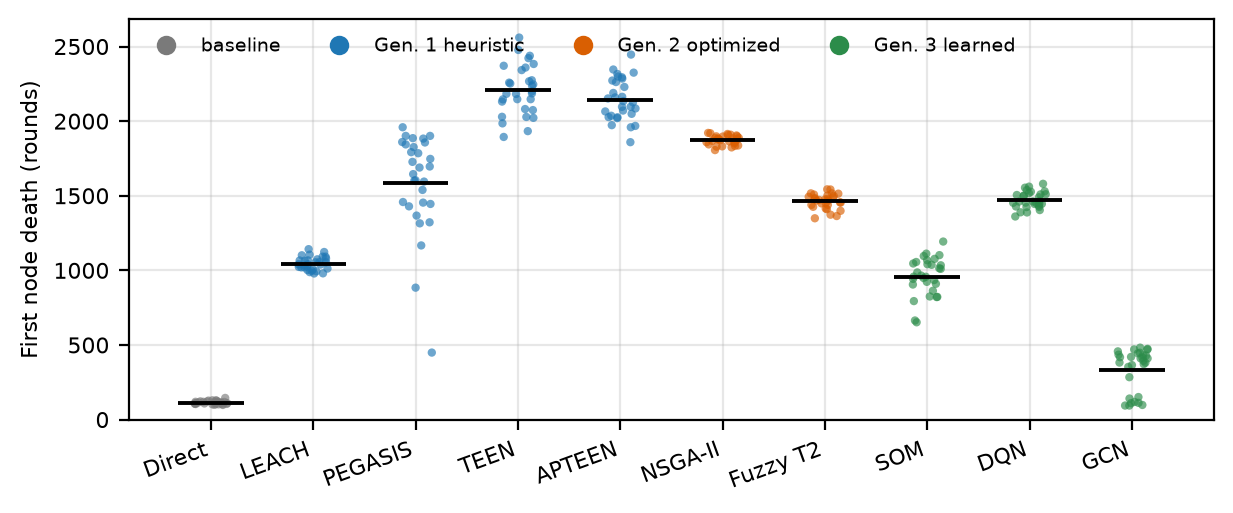
\includegraphics[width=\columnwidth]{figB_fnd_distribution.png}
\caption{First node death per trial, lossy channel, all 30 paired trials shown
individually rather than as a mean and a deviation. The reactive pair leads, the
GCN is visibly bimodal, and PEGASIS carries one topology at 449 rounds against a
body near 1{,}800. A mean and standard deviation would describe none of these
three distributions correctly.}
\label{fig:fnd-dist}
\end{figure}

Table~\ref{tab:lifetime} gives the full lossy-channel results. Against LEACH,
with paired permutation testing and Holm correction across the family, every
protocol differs significantly. The reactive pair leads on first death by a wide
margin, TEEN at 2{,}208 rounds with $\Delta = +1{,}163$, followed by NSGA-II at
1{,}873 ($\Delta = +827$), PEGASIS at 1{,}588, the DQN at 1{,}472 and the fuzzy
system at 1{,}462. Two protocols are significantly worse than LEACH: the
self-organizing map at 959 and the GCN at 335.

Three observations survive scrutiny and are worth stating separately from the
ranking.

NSGA-II posts both the best non-reactive first death and the tightest spread of
any of the nine clustering protocols, with a standard deviation of 31 rounds
against LEACH's 43, the DQN's 55 and PEGASIS's 331. Its advantage holds in both
channel configurations. But its convergence is modest, and we report that as a
finding rather than suppress it. Over the logged mid-run reclustering, the
population's best round-energy objective improves by 1.76\% and its best
minimum-head-energy objective by 3.61\%, while only cluster-size balance moves
substantially, from 2.99 to 1.85 for the population best and from 9.19 to 5.58
at the knee point. With five heads drawn from a hundred candidates, random
initialization already lands near a good solution. NSGA-II's advantage here
should therefore not be attributed to the sophistication of the search.

PEGASIS has by far the largest first-death variance of any protocol, 331 rounds
against a typical 30 to 60. A greedy chain is sensitive to where the topology
happens to place its outliers, and a single badly positioned node changes the
chain's whole cost structure; one trial gives 449 rounds against a body near
1{,}800. Its half-death figure, by contrast, has a standard deviation of 9
rounds, the tightest in the study, because once the chain has been rebuilt a few
times its structure becomes topology-insensitive.

The GCN's first death is not merely poor but bimodal. Across the first five
seeds it records 448, 394, 418, 112 and 98 rounds, and over all 30 trials eight
fall between 94 and 151 while the remaining twenty-two fall between 284 and 482.
A mean of 335 with a standard deviation of 142 describes neither mode.
Fig.~\ref{fig:fnd-dist} shows the shape, and
Section~\ref{sec:credit} explains it.

\subsection{A Conclusion the Channel Sweep Retracts}
\label{sec:retraction}

\begin{table*}[!t]
\caption{First-node-death difference against LEACH, in rounds, under both channel configurations. Paired sign-flip permutation test (20\,000 permutations) with paired-bootstrap confidence intervals, Holm-corrected across the nine comparisons within each channel. \textbf{Fuzzy T2 and DQN are significant under loss and not significant without it}, which is the study's central negative result.}
\label{tab:paired-fnd}
\centering
\begin{tabular}{lrcrrcr}
\toprule
& \multicolumn{3}{c}{Lossy channel} & \multicolumn{3}{c}{Ideal channel} \\
\cmidrule(lr){2-4}\cmidrule(lr){5-7}
Protocol & $\Delta$FND & 95\% CI & $p_{\mathrm{Holm}}$ & $\Delta$FND & 95\% CI & $p_{\mathrm{Holm}}$ \\
\midrule
Direct (no clustering) & -932 & [-944, -919] & 0.00045 & -1,153 & [-1,162, -1,144] & 0.00045 \\
PEGASIS & +542 & [+418, +647] & 0.00045 & +188 & [+78, +293] & 0.009 \\
TEEN & +1,163 & [+1,109, +1,217] & 0.00045 & +2,593 & [+2,542, +2,647] & 0.00045 \\
APTEEN & +1,099 & [+1,055, +1,143] & 0.00045 & +2,434 & [+2,392, +2,480] & 0.00045 \\
NSGA-II & +827 & [+811, +844] & 0.00045 & +482 & [+471, +493] & 0.00045 \\
Fuzzy T2 & +417 & [+393, +440] & 0.00045 & +17 & [+0, +34] & 0.119 \\
SOM & -87 & [-135, -41] & 0.001 & -399 & [-443, -357] & 0.00045 \\
DQN & +426 & [+404, +450] & 0.00045 & +22 & [-4, +49] & 0.124 \\
GCN & -710 & [-764, -660] & 0.00045 & -1,140 & [-1,193, -1,090] & 0.00045 \\
\bottomrule
\end{tabular}
\end{table*}

\begin{table}[!t]
\caption{Where the energy goes and where the heads sit, measured by the engine's own accounting categories (seed 0, 1100 rounds). Packet error is near zero below 120~m, so the \emph{mean} head distance cannot explain the retry gap --- every mean is below that. The tail can: across the six single-hop protocols, the share of head-rounds beyond 120~m predicts retry energy share with $r = 0.95$. PEGASIS is the exception that proves the rule: its leader rotates uniformly and 30\% of leader-rounds sit beyond 120~m, yet it retries barely at all, because only the leader ever faces the sink.}
\label{tab:energy-split}
\centering
\begin{tabular}{lrrrrr}
\toprule
Protocol & Retry & Control & \multicolumn{2}{c}{Head-to-sink (m)} & Heads $>$120 m \\
\cmidrule(lr){4-5}
 & (\%) & (\%) & mean & p90 & (\% of rounds) \\
\midrule
LEACH & 6.39 & 12.73 & 102.1 & 143.5 & 29.9 \\
PEGASIS & 1.39 & 4.38 & 102.2 & 143.5 & 30.0 \\
SOM & 5.28 & 2.38 & 102.8 & 136.4 & 31.1 \\
NSGA-II & 3.57 & 2.46 & 94.2 & 127.5 & 17.7 \\
Fuzzy T2 & 3.65 & 2.33 & 85.6 & 122.1 & 11.5 \\
DQN & 2.31 & 3.95 & 81.1 & 111.2 & 5.1 \\
GCN & 2.25 & 3.85 & 77.1 & 104.6 & 3.2 \\
\bottomrule
\end{tabular}
\end{table}


Applying the decision rule of Section~\ref{sec:channel-pair} to the 30-run
sweep, one conclusion does not survive, and it is a load-bearing one. On the
lossy channel the fuzzy system and the DQN improve first death over LEACH by 417
and 426 rounds respectively, both at the corrected significance floor of
$p_{\mathrm{Holm}} = 0.00045$. On the ideal channel the same comparisons give 17
and 22 rounds at $p_{\mathrm{Holm}} = 0.119$ and $0.124$, which is not
significant. Remove packet loss and both protocols become statistically
indistinguishable from LEACH on the metric this literature most often reports.
Table~\ref{tab:paired-fnd} gives both channels side by side.

We measured the mechanism rather than arguing it, and the measurement rules out
the explanation we expected. Table~\ref{tab:energy-split} splits each protocol's
energy by accounting category over a single seed and reports the full
distribution of head-to-sink distance in the same run, not only its mean.

\begin{figure}[!t]
\centering
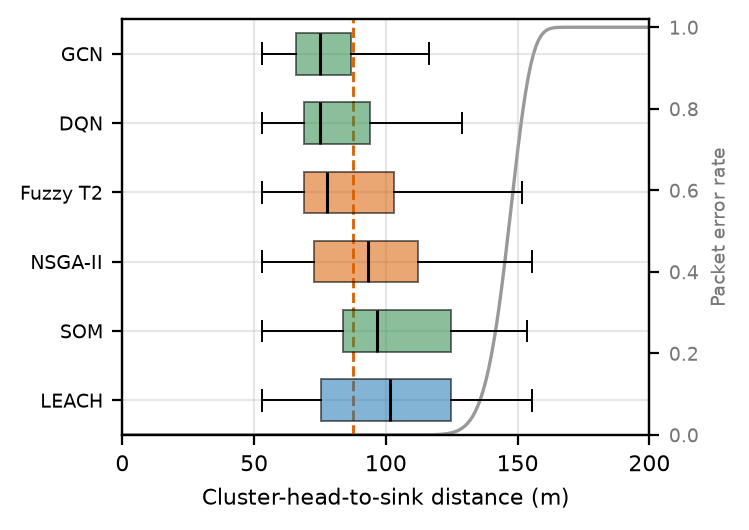
\includegraphics[width=\columnwidth]{figF_head_distance.png}
\caption{Distribution of head-to-sink distance per protocol, drawn over the
packet-error curve. Every protocol's \emph{mean} falls in the flat region where
packet error is effectively zero, so the mean cannot be what drives the retry
gap. The distributions differ in their upper tails, and only the tails reach the
waterfall.}
\label{fig:head-dist}
\end{figure}

The obvious reading of these numbers would be that LEACH's average cluster head
sits at 102.1~m, past the 87.7~m crossover and therefore onto the fourth-power
branch, while the DQN's sits at 81.1~m. That is true, and it explains part of
the difference in raw transmit energy, but it cannot explain the
retransmissions. Packet error is $2.6\times10^{-8}$ at 100~m and does not reach
$10^{-3}$ until 120~m, and every protocol in Table~\ref{tab:energy-split} has a
mean head distance below 120~m. A protocol whose heads all sat at the mean would
retry essentially never.

What separates them is the upper tail, shown in Fig.~\ref{fig:head-dist}. LEACH
spends 29.9\% of its head-rounds beyond 120~m and 6.39\% of its budget on
retransmissions. The DQN spends 5.1\% of its head-rounds beyond 120~m and 2.31\%
on retransmissions. Across the six single-hop protocols the share of head-rounds
beyond 120~m correlates with retry energy share at $r = 0.95$. The mean distance
correlates almost as strongly, at $r = 0.93$, because the two quantities are
collinear; the reason to prefer the tail is not a better fit but that only the
tail lies in the region where packets actually fail.

\begin{figure}[!t]
\centering
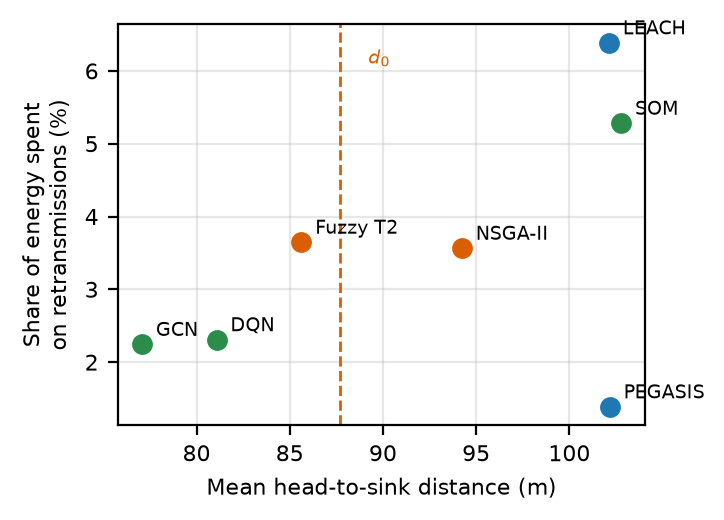
\includegraphics[width=\columnwidth]{figC_mechanism.png}
\caption{Retry energy share against the share of head-rounds beyond 120~m, lossy
channel, seed 0. The six single-hop protocols line up at $r = 0.95$. PEGASIS,
plotted separately, has the same 30\% tail as LEACH and almost no retry cost,
because only its leader ever faces the sink.}
\label{fig:mechanism}
\end{figure}

PEGASIS is the exception that fixes the scope of the claim, and we state it
rather than exclude it quietly. Its leader rotates uniformly over chain
positions, so its leader-distance distribution is identical to the node
distribution and 30.0\% of leader-rounds sit beyond 120~m, the same as LEACH.
Yet it retries on only 1.39\% of its budget. Including it drops the correlation
from 0.95 to 0.50. The reason is structural: in a chain, exactly one node faces
the sink per round while every other transmission is a short hop to a neighbor,
so the tail of the sink-facing distribution is paid once per round instead of
five times. The claim is therefore specific to single-hop clustered protocols,
where every head pays the sink hop, and Fig.~\ref{fig:mechanism} plots it that
way.

The honest claim is therefore narrower, and more interesting, than ``the
soft-computing and learned protocols cluster better''. Their demonstrable skill
is keeping the far tail of the head-to-sink hop out of the error waterfall, and
that skill pays only in proportion to how lossy that hop is. Delete the loss by
making the channel lossless and the advantage disappears. The same table shows
LEACH's compensating strength: it consumes 20\% more total energy than the DQN
yet matches its first death on a clean channel, because its epoch rule rotates
head duty perfectly.

The retraction is specific to first death and we do not overstate it. On area
under the living-node curve and on readings delivered, every protocol's
difference from LEACH is significant at the corrected floor in both channels, in
the same direction and at similar magnitude; the fuzzy system gains 24{,}793
node-rounds on the lossy channel and 22{,}120 on the ideal.
Table~\ref{tab:paired-robust} gives these. The correct statement is that the
advantage in overall survival and in data delivered is robust to the channel,
and only the advantage in first death is not. First death is a single order
statistic and the most fragile of the four lifetime measures.

\begin{table}[!t]
\caption{Survival and delivery differences against LEACH under both channels. Unlike first node death (Table~\ref{tab:paired-fnd}), every one of these gaps holds in both configurations, so these are the conclusions the study can state without a channel caveat.}
\label{tab:paired-robust}
\centering
\begin{tabular}{lrrrr}
\toprule
& \multicolumn{2}{c}{Lossy} & \multicolumn{2}{c}{Ideal} \\
\cmidrule(lr){2-3}\cmidrule(lr){4-5}
Protocol & $\Delta$ ($\times 10^3$) & $p_{\mathrm{Holm}}$ & $\Delta$ ($\times 10^3$) & $p_{\mathrm{Holm}}$ \\
\midrule
\multicolumn{5}{l}{\textit{AUC}} \\
\quad Direct (no clustering) & -35.1 & 0.0004 & -32.8 & 0.0004 \\
\quad PEGASIS & +49.2 & 0.0004 & +44.5 & 0.0004 \\
\quad TEEN & +368.3 & 0.0004 & +389.6 & 0.0004 \\
\quad APTEEN & +351.3 & 0.0004 & +371.7 & 0.0004 \\
\quad NSGA-II & +33.5 & 0.0004 & +31.7 & 0.0004 \\
\quad Fuzzy T2 & +24.8 & 0.0004 & +22.1 & 0.0004 \\
\quad SOM & +29.7 & 0.0004 & +29.2 & 0.0004 \\
\quad DQN & +25.0 & 0.0004 & +22.5 & 0.0004 \\
\quad GCN & +13.1 & 0.0004 & +11.1 & 0.0004 \\
\addlinespace
\multicolumn{5}{l}{\textit{Readings}} \\
\quad Direct (no clustering) & -18.5 & 0.0004 & -31.8 & 0.0004 \\
\quad PEGASIS & +35.6 & 0.0004 & +44.2 & 0.0004 \\
\quad TEEN & -88.1 & 0.0004 & -106.0 & 0.0004 \\
\quad APTEEN & -84.0 & 0.0004 & -101.3 & 0.0004 \\
\quad NSGA-II & +33.2 & 0.0004 & +32.2 & 0.0004 \\
\quad Fuzzy T2 & +28.8 & 0.0004 & +22.4 & 0.0004 \\
\quad SOM & +29.2 & 0.0004 & +29.3 & 0.0004 \\
\quad DQN & +26.9 & 0.0004 & +22.5 & 0.0004 \\
\quad GCN & +16.2 & 0.0004 & +9.8 & 0.0004 \\
\bottomrule
\end{tabular}
\end{table}

\begin{table}[!t]
\caption{Every ranking that moves when the channel changes: 4 of 40 protocol--metric ranks. All are single-place swaps between adjacent protocols. Ordering is therefore stable; it is the \emph{significance} of specific first-node-death gaps that is not (Table~\ref{tab:paired-fnd}).}
\label{tab:robustness}
\centering
\begin{tabular}{llrrr}
\toprule
Metric & Protocol & Lossy rank & Ideal rank & Shift \\
\midrule
hnd & Fuzzy T2 & 4 & 5 & +1 \\
hnd & SOM & 5 & 4 & -1 \\
readings\_delivered\_total & Fuzzy T2 & 4 & 5 & +1 \\
readings\_delivered\_total & DQN & 5 & 4 & -1 \\
\bottomrule
\end{tabular}
\end{table}


Across all forty protocol-metric rankings, four ranks move between channel
configurations, and both moving pairs are near-ties between adjacent protocols
(Table~\ref{tab:robustness}). The ordering is therefore stable. What is not
stable is the statistical significance of specific first-death gaps.

\subsection{What Temporal Credit Assignment Buys}
\label{sec:credit}

\begin{table}[!t]
\caption{Head-duty concentration over 1100 rounds (seed 0), in rounds served as cluster head per node. LEACH's 55 is exact rather than approximate: its epoch mechanism elects every node exactly once per 20 rounds. GCN's busiest node serves 13.6 times as often, which is the direct cause of its early first node death (Table~\ref{tab:lifetime}) --- it does not choose badly, it chooses the same good node until that node dies.}
\label{tab:head-rotation}
\centering
\begin{tabular}{lrrrr}
\toprule
Protocol & Busiest node & Median & Never served & Gini \\
\midrule
LEACH & 55 & 55 & 0 & 0.001 \\
PEGASIS & 11 & 11 & 0 & 0.000 \\
NSGA-II & 95 & 60 & 0 & 0.207 \\
Fuzzy T2 & 360 & 40 & 4 & 0.416 \\
SOM & 175 & 50 & 10 & 0.393 \\
DQN & 223 & 38 & 16 & 0.476 \\
GCN & 750 & 16 & 13 & 0.700 \\
\bottomrule
\end{tabular}
\end{table}


The DQN and the GCN consume identical inputs and differ only in architecture and
training signal, so the gap between them isolates one variable. Over the 30
paired trials the DQN's first death ranges from 1{,}361 to 1{,}580, a spread of
219 rounds with a standard deviation of 55. The GCN's ranges from 94 to 482, a
spread of 388 with a standard deviation of 142, and it is bimodal rather than
merely wide.

\begin{figure}[!t]
\centering
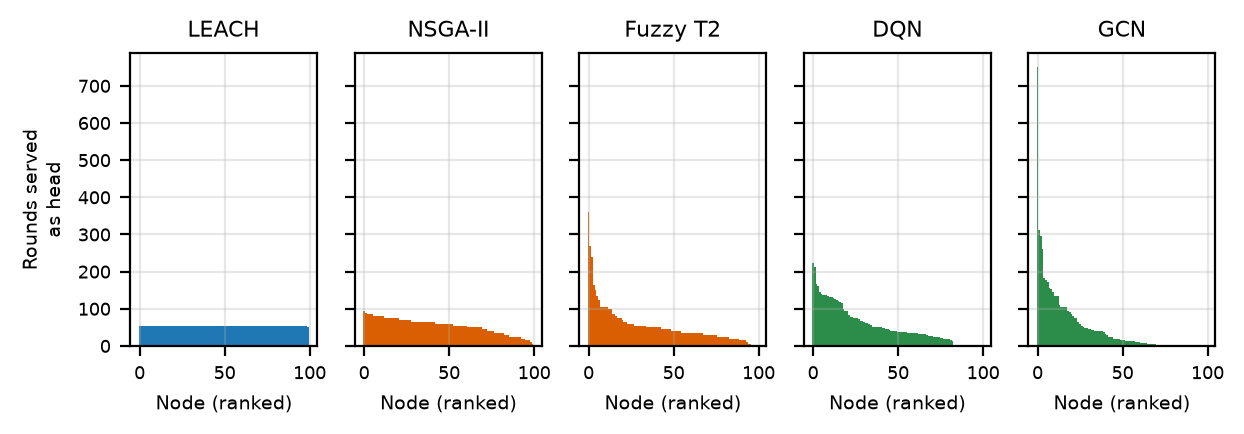
\includegraphics[width=\columnwidth]{figG_head_rotation.png}
\caption{Rounds served as cluster head per node over 1{,}100 rounds, seed 0,
sorted. LEACH's epoch rule produces a flat line at exactly 55. The GCN's curve is
the opposite extreme: it concentrates 750 rounds of head duty on one node while
13 nodes never serve at all, which is what its single-round objective is
indifferent to.}
\label{fig:rotation}
\end{figure}

Table~\ref{tab:head-rotation} measures why over 1{,}100 rounds on seed 0. The
GCN's busiest node serves as cluster head for 750 of those rounds against
LEACH's 55, a factor of 13.6, and its Gini coefficient over head duty is 0.700
against LEACH's 0.001. Thirteen of its nodes never serve at all, and its median
node serves 16 rounds. It does not choose badly. It repeatedly chooses the same
genuinely good node until that node dies, which is exactly the failure a
single-round objective cannot see. The DQN, with the same four features
including rounds since last serving as head, concentrates far less: 223 rounds
on its busiest node and a Gini of 0.476. Fig.~\ref{fig:rotation} shows the two
curves against LEACH's flat line.

This is the paper's cleanest controlled contrast. The GCN can see rotation state
in its input. What it lacks is any term in its loss that rewards deferring cost
to extend lifetime, and the cost of that omission is a first death 3.1 times
earlier than LEACH's. It is also the only protocol to lose to LEACH on first
death in both channel configurations by a wide margin.

\subsection{Delivery and the Reactive Tradeoff}

TEEN and APTEEN dominate every lifetime metric and fail to reach full depletion
within the 7{,}000-round cap in all 30 trials, so their last-death figures are
lower bounds. Their area under the living-node curve is 3.2 times LEACH's. This
is not free. Their data yield is 0.109 and 0.121 against roughly 0.9 for the
proactive protocols, and they deliver 58{,}551 and 62{,}579 readings against
LEACH's 146{,}616. They survive by not reporting, and their reporting rate,
0.15 and 0.17 of rounds respectively, is the quantity that makes the lifetime
figure interpretable. Reported without it, their lifetime is not a result about
clustering at all.

Table~\ref{tab:delivery} also shows why packets at the base station must not be
compared across protocols. PEGASIS delivers 182{,}179 readings in 2{,}272
packets, an aggregation ratio of 80, while the direct baseline delivers 128{,}075
readings in 128{,}075 packets. On a packet count PEGASIS looks like the worst
protocol in the study and on readings it is the best.

\subsection{Cost and Latency}

\begin{table*}[!t]
\caption{Cost, lossy channel. Counted operations are the honest cross-protocol comparison; wall-clock setup time reflects implementation quality as much as algorithm design and is reported separately for that reason. DQN and GCN setup times are inference only: their one-off offline training is not included here (Section~\ref{sec:validity}).}
\label{tab:cost}
\centering
\begin{tabular}{llrrrrrr}
\toprule
Protocol & Gen. & Latency & p95 & Control pkts & Ops per & Setup & Peak mem \\
 & & (ms) & (ms) & ($\times 10^3$) & round & (ms) & (MB) \\
\midrule
Direct (no clustering) & -- & 600 & 1,488 & 0.0 & 0 & 0.00 & 6.0 \\
LEACH & G1 & 274 & 837 & 171.6 & 329 & 0.82 & 1.7 \\
PEGASIS & G1 & 1,045 & 1,626 & 213.9 & 59 & 0.05 & 1.5 \\
TEEN & G1 & 419 & 990 & 573.9 & 307 & 0.83 & 5.1 \\
APTEEN & G1 & 407 & 979 & 554.3 & 296 & 0.80 & 5.1 \\
NSGA-II & G2 & 387 & 573 & 10.8 & 86,348 & 102.89 & 2.1 \\
Fuzzy T2 & G2 & 401 & 1,028 & 9.7 & 2,301 & 5.14 & 1.6 \\
SOM & G3 & 388 & 538 & 10.7 & 6,194 & 38.28 & 2.0 \\
DQN & G3 & 402 & 918 & 11.9 & 8,210 & 0.52 & 1.7 \\
GCN & G3 & 392 & 981 & 12.2 & 5,454 & 0.88 & 2.3 \\
\bottomrule
\end{tabular}
\end{table*}


Latency separates the protocols structurally. The clustered protocols sit
between 387 and 419~ms mean, LEACH is lowest at 274~ms because its stochastic
election produces smaller average clusters, and PEGASIS is an outlier at
1{,}045~ms mean and 1{,}626~ms at the 95th percentile. Chain depth is the
dominant latency cost and no amount of energy efficiency compensates for it. The
ordering is structurally correct, but the absolute figures are lower bounds,
since the model contains no queueing or contention delay.

Computational cost is where the three measurement notions of
Section~\ref{sec:metrics} disagree most sharply, which is the argument for
keeping them separate. NSGA-II costs 102.9~ms per round of setup against LEACH's
0.82~ms, a factor of 126, and 86{,}348 counted operations against 329, a factor
of 262. The self-organizing map is second at 38.3~ms. But the ordering by
counted operations and by wall-clock is not the same. The DQN performs 8{,}210
counted operations per round in 0.52~ms, while the fuzzy system performs 2{,}301
in 5.14~ms. The DQN does 3.6 times the algorithmic work in a tenth of the time,
because its work is a dense matrix product and the fuzzy system's is an
iterative type-reduction loop. Reporting either number alone would invert the
comparison.

Control traffic differs by more than an order of magnitude across classes:
573{,}870 packets for TEEN and 171{,}644 for LEACH against 9{,}657 to 12{,}216
for the centralized five. That gap is substantially an artifact of the
accounting model rather than of clustering quality, and
Section~\ref{sec:validity} quantifies it.

\subsection{Node Count, Field Area, and the Regime Boundary}
\label{sec:scale}

\begin{table*}[!t]
\caption{First node death (rounds) across node counts and field areas, lossy channel, 15 paired runs per cell.}
\label{tab:scale-fnd}
\centering
\begin{tabular}{llrrrrrrrrr}
\toprule
  &   & \multicolumn{3}{c}{50$\times$50 m} & \multicolumn{3}{c}{100$\times$100 m} & \multicolumn{3}{c}{150$\times$150 m} \\
\cmidrule(lr){3-5}\cmidrule(lr){6-8}\cmidrule(lr){9-11}
Protocol & Gen. & $N{=}50$ & $N{=}100$ & $N{=}150$ & $N{=}50$ & $N{=}100$ & $N{=}150$ & $N{=}50$ & $N{=}100$ & $N{=}150$ \\
\midrule
Direct (no clustering) & -- & 2,178 & 1,943 & 1,677 & 120 & 112 & 111 & 23 & 22 & 22 \\
LEACH & G1 & 1,791 & 1,617 & 1,586 & 641 & 1,034 & 1,085 & 155 & 303 & 354 \\
PEGASIS & G1 & 2,097 & 2,114 & 2,062 & 1,550 & 1,610 & 1,517 & 663 & 815 & 720 \\
TEEN & G1 & 6,808 & 5,899 & 5,186 & 2,028 & 2,201 & 2,064 & 425 & 550 & 532 \\
APTEEN & G1 & 6,831 & 5,684 & 5,002 & 1,947 & 2,141 & 1,992 & 427 & 519 & 527 \\
NSGA-II & G2 & 2,184 & 2,173 & 2,160 & 1,818 & 1,872 & 1,865 & 717 & 1,052 & 1,077 \\
Fuzzy T2 & G2 & 1,656 & 1,685 & 1,698 & 1,379 & 1,454 & 1,470 & 381 & 393 & 577 \\
SOM & G3 & 1,382 & 1,280 & 1,296 & 1,153 & 965 & 994 & 591 & 342 & 328 \\
DQN & G3 & 1,500 & 1,628 & 1,677 & 1,296 & 1,478 & 1,537 & 454 & 559 & 833 \\
GCN & G3 & 200 & 208 & 138 & 152 & 371 & 305 & 71 & 158 & 82 \\
\bottomrule
\end{tabular}

{\footnotesize The base station scales with the field at $(W/2,\,1.5W)$, so field size sets channel severity as well as area. Node-to-sink distance by field size --- 50$\times$50~m: mean 52~m, 0\% of nodes beyond 120~m; 100$\times$100~m: mean 104~m, 33\% of nodes beyond 120~m; 150$\times$150~m: mean 156~m, 75\% of nodes beyond 120~m. At $50\times50$~m no link reaches the error waterfall at all, which is why the advantage of the optimized and learned protocols over LEACH collapses there.\par}
\end{table*}

\begin{table}[!t]
\caption{Cells ordered by node density. If density drove lifetime the rows would trend with it; they do not --- the numbers track the mean sink distance column instead. Averaged over all ten protocols, tripling the node count changes first node death by a factor of 0.88--1.26, while tripling the field side changes it by a factor of 5--7. The two cells closest in density (50 and 44 nodes/ha) differ by 1.7$\times$ for NSGA-II, 2.1$\times$ for LEACH and 5.5$\times$ for direct transmission. Note also that \emph{clustering only pays once the sink is far}: in the $50\times50$~m rows the no-clustering baseline outlives LEACH.}
\label{tab:scale-density}
\centering
\begin{tabular}{llrrrrr}
\toprule
$N$ & Field (m) & Density & Mean sink & \multicolumn{3}{c}{First node death (rounds)} \\
\cmidrule(lr){5-7}
 & & (nodes/ha) & dist.\ (m) & Direct & LEACH & NSGA-II \\
\midrule
50 & 150$\times$150 & 22 & 156 & 23 & 155 & 717 \\
100 & 150$\times$150 & 44 & 156 & 22 & 303 & 1,052 \\
50 & 100$\times$100 & 50 & 104 & 120 & 641 & 1,818 \\
150 & 150$\times$150 & 67 & 156 & 22 & 354 & 1,077 \\
100 & 100$\times$100 & 100 & 104 & 112 & 1,034 & 1,872 \\
150 & 100$\times$100 & 150 & 104 & 111 & 1,085 & 1,865 \\
50 & 50$\times$50 & 200 & 52 & 2,178 & 1,791 & 2,184 \\
100 & 50$\times$50 & 400 & 52 & 1,943 & 1,617 & 2,173 \\
150 & 50$\times$50 & 600 & 52 & 1,677 & 1,586 & 2,160 \\
\bottomrule
\end{tabular}
\end{table}


The headline study measures one deployment. The $3\times3$ sweep of
Section~\ref{sec:scale-design} asks which of its conclusions are about
clustering and which are about that deployment.
Table~\ref{tab:scale-fnd} gives first node death in all nine cells and
Table~\ref{tab:scale-density} reorders the same cells by node density.

\begin{figure}[!t]
\centering
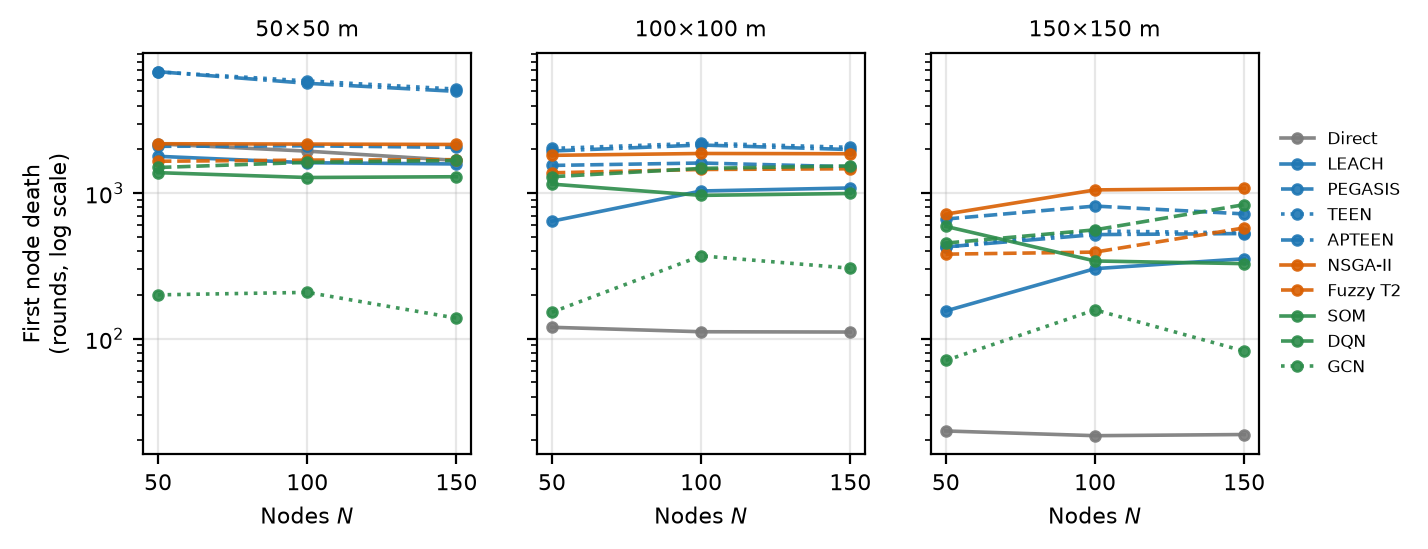
\includegraphics[width=\columnwidth]{figD_scale_fnd.png}
\caption{First node death across the nine cells, log scale, color by
generation. Moving between field sizes shifts every protocol by roughly an order
of magnitude; moving between node counts within a field size barely moves
anything. The reactive pair reverses rank between the smallest and largest
fields.}
\label{fig:scale-fnd}
\end{figure}

\emph{Area dominates node count by roughly five to one.} Averaged over all ten
configurations, tripling the node count changes first node death by a factor of
0.88 to 1.26, while tripling the field side changes it by a factor of 5 to 7.
Fig.~\ref{fig:scale-fnd} shows the separation directly.

\emph{The driver is distance to the sink, not density.}
Table~\ref{tab:scale-density} orders the cells by node density, and if density
were the cause the rows would trend with it. They do not; they track the mean
sink distance column instead. The two cells closest in density, 50 and 44
nodes per hectare, differ by 1.7 times for NSGA-II, 2.1 times for LEACH and 5.5
times for direct transmission, because one has its sink 104~m away and the other
156~m. We note the limitation this rests on: the grid was not designed to hold
density constant, so no two cells match exactly, and this is a near-match rather
than a controlled contrast. The effect sizes differ by enough that the
conclusion is not sensitive to the gap, but the design does not license a
stronger statement.

\begin{figure}[!t]
\centering
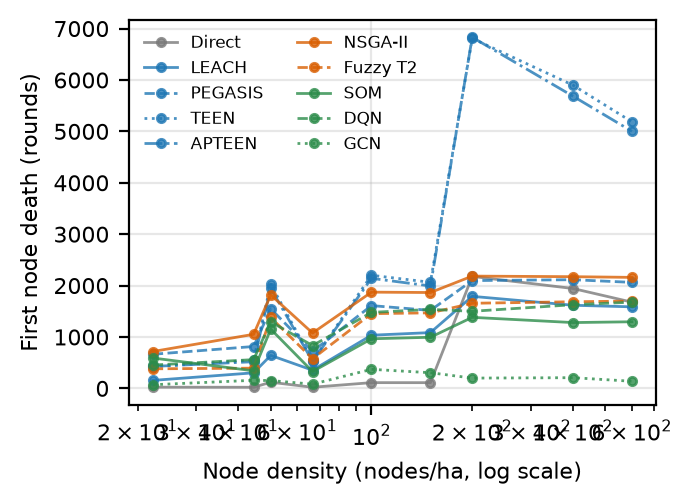
\includegraphics[width=\columnwidth]{figE_scale_density.png}
\caption{First node death against node density, with points coloured by field
size. Density spans a factor of 27 across the grid and explains almost none of
the variation; the three field-size bands separate cleanly instead.}
\label{fig:scale-density}
\end{figure}

\emph{Clustering is harmful when the sink is close.} In the $50\times50$~m
field, where the mean node-to-sink distance is 52~m and no node lies beyond
120~m, LEACH's first node death relative to no clustering at all is a factor of
0.82, 0.83 and 0.95 at $N = 50$, 100 and 150. The no-clustering baseline outlives
LEACH in all three cells, on area under the living-node curve as well as on first
death. At $100\times100$~m the same ratios are 5.4, 9.3 and 9.8, and at
$150\times150$~m they are 6.7, 13.8 and 16.1. The opening result of
Section~\ref{sec:results} is therefore not a statement about clustering as such
but about an operating regime: clustering pays once the sink hop is expensive
enough to be worth aggregating away, and not before.

\emph{The channel retraction reproduces from an independent direction.} In the
$50\times50$~m field the DQN's first-death advantage over LEACH falls to $+10$
rounds at $N = 100$ and to $-291$ at $N = 50$, against $+444$ at
$100\times100$~m; the fuzzy system falls to $+68$ and $-135$ against $+419$.
This is the same boundary found in Section~\ref{sec:retraction} by removing
packet loss, reached instead by moving the sink close enough that no link
reaches the waterfall. The fuzzy system is what makes the attribution safe: it
has no training of any kind, so its collapse cannot be a transfer failure and
must be a property of the environment. Since the DQN behaves the same way, the
DQN's collapse is a property of the environment too.

\emph{Rankings are partly stable and the exceptions are informative.} NSGA-II
holds ranks 1 to 3 in every cell, takes rank 1 in all three $150\times150$~m
cells, and beats LEACH in all nine by margins from $+394$ to $+1{,}177$ rounds.
The GCN holds ranks 9 to 10 everywhere. Against those, the DQN's rank improves
monotonically as the field grows, and TEEN and APTEEN reverse outright, from
ranks 1 and 2 in the two smaller fields to ranks 4 to 6 at $150\times150$~m
where NSGA-II and PEGASIS overtake them. Rankings by area under the living-node
curve are considerably more stable than by first death, with every protocol
except the direct baseline moving at most four places.

\emph{The frozen policies do not collapse off their training distribution.}
The DQN and the GCN carry $N = 100$, $100\times100$~m weights into all nine
cells with no retraining. Neither fails catastrophically, and the GCN's deficit
against LEACH actually shrinks as the field grows, from between $-1{,}409$ and
$-1{,}591$ rounds in the smallest field to between $-84$ and $-272$ in the
largest, although it remains worse than LEACH in every cell. This is weaker
evidence than a retrained comparison would give, and it is not a claim that
these policies are scale-invariant. It is a claim that their reported advantage
is not an artifact of evaluating them only at the point where they were trained.

Two of our five pre-registered expectations about this sweep were wrong, and we
report both. We expected the generational gap to widen at $150\times150$~m; it
narrows there as well as at $50\times50$~m, so the gap is largest in the middle
cell. We expected node density to matter; it does not.

\section{Threats to Validity}
\label{sec:validity}

Every result in Section~\ref{sec:results} depends on choices that a reader
cannot see in the numbers. This section states them, ordered by how far each
could move a conclusion, and it names the one that could move the most first.

\subsection{The Control-Traffic Subsidy}
\label{sec:subsidy}

Centralized protocols are charged nothing for the uplink that informs the sink
of node state. This is the largest single confound in the study and it favors
five of the ten configurations.

The justification is quantitative. A separate 200-bit status report per node per
round, over a sink distance above 100~m and therefore on the fourth-power
branch, costs roughly $3.6\times10^{-5}$~J per node per round, accumulating to
about a quarter of the entire 1~J budget across the round cap. Charging it would
sink all five centralized protocols for a reason unconnected to whether their
clustering decisions are any good, and the piggyback assumption is standard in
the centralized-clustering literature. But a defensible modeling choice is still
a modeling choice, and its magnitude belongs in the results rather than in a
footnote.

Measured over the full sweep, LEACH spends 12.73\% of its consumed energy on
control traffic against 2.33\% for the fuzzy system, 2.46\% for NSGA-II, 2.38\%
for the map, 3.95\% for the DQN and 3.85\% for the GCN. The subsidy is therefore
worth roughly nine to ten percentage points of the total budget. In packet terms
the gap is starker still, 171{,}644 control packets for LEACH and 573{,}870 for
TEEN against 9{,}657 to 12{,}216 for the centralized five, but the packet gap
overstates the effect, since control packets are a fifth the size of data packets
and most are short-range.

Two consequences follow. First, a claim of the form ``NSGA-II extends first
death by 80\% over LEACH'' conflates clustering quality with an accounting
convention and should not be made without qualification. Second, the reliable
comparisons in this paper are the within-class ones: centralized against
centralized, distributed against distributed, with the chain protocol comparing
cleanly to neither. Section~\ref{sec:results}'s strongest results, the
channel-conditional retraction and the DQN-versus-GCN rotation contrast, are both
within-class and are unaffected.

The clean resolution is an ablation that charges the uplink honestly and re-runs
the sweep. It would convert this caveat into a measurement, and it is the single
most valuable follow-up this codebase supports. It has not been run.

\subsection{Transmit Power Is Bracketed, Not Swept}

Section~\ref{sec:retraction} treats the channel comparison as a result, which it
is, but the design bounds what it establishes. Two configurations bracket a
continuum; they do not trace it. The lossy setting places the sink hop near the
packet-error waterfall and the ideal setting removes loss entirely, so a
conclusion stable across both is stable across that interval. A transmit power
between them, or above the lossy setting, would produce intermediate behavior
this study does not measure. A three-point or four-point sweep over transmit
power would trace the curve properly and would show where the fuzzy system's and
the DQN's first-death advantage over LEACH actually crosses the significance
threshold. That sweep has not been run.

The scale sweep of Section~\ref{sec:scale} partially compensates, because moving
the sink changes how much of the node population sits in the waterfall and
reaches the same boundary from a different direction. It is not a substitute:
field size changes area and channel severity together, so it identifies the
boundary without isolating the parameter.

Related parameters are equally unspecified in the source material and equally
consequential: the path-loss exponent, the shadowing standard deviation, the
noise floor and the retry budget. We used conventional values for 2.4~GHz
outdoor short-range links~\cite{rappaport2002wireless,ieee802154} and published
the resulting packet-error curve so that the choice is auditable, but we did not
vary them.

\subsection{The Pre-Training Asymmetry}

The DQN and the GCN arrive pre-trained; the other seven protocols do not. Three
distinct caveats follow and all belong in any citation of these results.

Their reported setup time and operation counts are inference costs only.
Training is real, is paid once, and is reported separately. It must not be read
as free.

The seven non-learned protocols receive no equivalent offline preparation. This
is a fair comparison of a deployed system and it is not an apples-to-apples
algorithmic comparison. Both statements are true simultaneously, and which one
matters depends on the question being asked.

Generalization is now measured rather than assumed, but only in one direction.
The evaluation seeds are disjoint from the training seeds, so the headline
result is not memorization. The scale sweep additionally carries the frozen
$N = 100$, $100\times100$~m weights into eight cells the policies never saw, and
neither policy collapses; the GCN's deficit against LEACH even narrows as the
field grows. What that does not establish is how these policies would compare
against retrained versions of themselves, or how they behave under a sink
placement that is not geometrically similar to the training one. Every cell in
the sweep keeps the base station at $(W/2, 1.5W)$.

\subsection{Modeling Simplifications}

The radio model accounts for transmit, receive and fusion energy and nothing
else. There is no idle-listening cost, no sleep-wake transition energy, no radio
startup and no processor energy. Idle listening frequently dominates real
deployments, and including it would compress the differences between all ten
configurations toward zero. Energy is a linear reservoir with no rate-capacity
effect, no recovery effect and no voltage cutoff.

Fusion is ideal. A head that receives any number of member packets emits exactly
one, so compression is lossless and free in bits. This systematically favors
high-fan-in structures, and PEGASIS most of all: its aggregation ratio of 80
readings per delivered packet is exactly the quantity this assumption idealizes.
The engine enforces the rule symmetrically, so no protocol can exploit it beyond
what its own topology allows, but the assumption still shapes the
chain-versus-cluster comparison more than any other single simplification.

There is no MAC layer. Scheduling is assumed perfect and collision-free, with no
contention, no hidden terminals, no inter-cluster interference and no capture
effect. Packet loss comes only from distance-dependent
error~\cite{zhao2003understanding,woo2003taming}. Adding interference would
penalize dense-cluster protocols relative to the chain and would make the number
of simultaneously active heads a variable this study cannot see. Latency inherits
the same limitation: it is analytic rather than queueing-based, retransmissions
cost energy but not modeled time, and the absolute figures in
Section~\ref{sec:results} are lower bounds whose ordering is meaningful and whose
magnitudes are not.

Everything is static. Nodes never move and fail only by depletion, so per-link
shadowing is drawn once and held fixed. There is no mobility, no node addition
and no environmental change across the run. The head-to-sink hop is single-hop
for nine of ten configurations, matching each protocol's original specification,
which leaves the chain as the sole multi-hop contrast.

Sensor data is a mean-reverting process rather than a real trace. The reactive
protocols' results are conditional on that model, and a bursty or spatially
correlated field would change them substantially. The thresholds were set
against the process's stationary distribution before any result was observed,
and were not adjusted afterward.

Finally, every protocol targets the same nominal head count but realizes it
differently, and LEACH's realized count is deliberately left stochastic. Part of
every observed difference is therefore attributable to realized cluster count
rather than to selection logic. Fixing the target isolates the question these
protocols actually differ on, namely which five of the roughly five heads
available should be chosen, but it does not eliminate the effect.

\subsection{Scope}

This study establishes results at one energy budget and one traffic model.
Network scale is now swept over three node counts and three field areas, but
within a single family of geometrically similar deployments, and three protocols
have complexity superlinear in node count. Node energy is homogeneous; the
configuration supports heterogeneity but it is disabled throughout. Every node
senses every round, with no duty cycling, event-driven traffic or query
workload. APTEEN's query facilities in particular are out of scope, and only its
reporting-frequency mechanism is modeled. There is no hardware testbed and no
measured trace; every number is simulation output under the assumptions above.

The scale sweep also carries one design limitation worth repeating here. Cells
were chosen to span node count and area independently, not to hold density
constant, so the finding that density does not drive lifetime rests on a close
pairing (50 against 44 nodes per hectare) rather than an exact match. The effect
sizes involved are large enough that a small density gap cannot account for
them, but a grid designed around density would settle the point more directly.

\subsection{On Not Calibrating}

No protocol was tuned to reproduce a published figure. Only protocol
descriptions, the radio model and simulation parameters were taken from prior
work; its numeric results were discarded before implementation began.
Disagreement with published tables is therefore expected and is not evidence of
error here.

The one place this commitment was tested is documented in
Section~\ref{sec:dqn-disclosure}. The DQN's discount factor and training length
were revised after an observed divergence, after which a stopping rule was fixed
in advance and the result recorded as final regardless of outcome. We state this
because the alternative, presenting the final hyperparameters as if they had been
the first, is the ordinary way such revisions disappear from a methods
section~\cite{henderson2018matters,pineau2021reproducibility}.

\section{Conclusion}
\label{sec:conclusion}

We built a single simulation engine in which nine clustering protocols spanning
twenty-five years of design practice execute under provably identical physical
conditions, and evaluated them over 600 runs across two channel configurations
and a further 1{,}350 runs across nine deployment scales. The engine owns energy
accounting, packet sizing, fusion charges, the channel and reading accounting; a
protocol returns only a cluster structure. Fairness is therefore a property of
the construction rather than of the authors' care, and it is verified by static
audit rather than asserted.

Five findings hold up.

Clustering does not extend network lifetime so much as redistribute it. LEACH
delays first node death by a factor of 9.2 over direct transmission while
bringing last death forward by nearly a third, because about a third of the
nodes lie close enough to the sink to transmit on the free-space branch and are
penalized rather than helped by rotation. No single lifetime figure summarizes
this, and the two most commonly reported figures order the protocols in opposite
directions.

The advantage of the soft-computing and learned protocols over LEACH in first
node death is conditional on the channel. Under packet loss the fuzzy system and
the Q-network improve on LEACH by 417 and 426 rounds; with loss removed the same
comparisons give 17 and 22 rounds and lose significance. Direct measurement of
the energy split shows why, and the explanation is not the one the mean
distances suggest. Every protocol's mean head-to-sink distance sits below 120~m,
where packet error is still effectively zero, so the mean cannot be the cause.
The tails differ instead: LEACH puts 29.9\% of its head-rounds beyond 120~m and
spends 6.39\% of its budget on retransmissions, against the Q-network's 5.1\% and
2.31\%. The demonstrable skill of the newer protocols is keeping the far tail of
the sink hop out of the error waterfall, and it pays in proportion to how lossy
that hop is. Their advantage in overall survival and in readings delivered is not
conditional; it holds in both configurations at the corrected significance floor.

The same boundary appears from an independent direction when the deployment
scales. Across three node counts and three field areas, tripling the node count
moves first node death by a factor of 0.88 to 1.26 while tripling the field side
moves it by a factor of 5 to 7, and cells of nearly equal density differ by up to
5.5 times. Distance to the sink is the variable, not density. In a
$50\times50$~m field, where nothing reaches the waterfall, the learned and
soft-computing advantages collapse exactly as they do when packet loss is
switched off, and clustering itself becomes counterproductive: the no-clustering
baseline outlives LEACH in all three of those cells.

Temporal credit assignment is worth measuring separately from representational
capacity. The Q-network and the graph network consume identical features and
differ only in architecture and training signal. The Q-network's first-death
distribution spans 219 rounds; the graph network's spans 388 and is bimodal, and
its busiest node serves as head 13.6 times as often as LEACH's while 13 nodes
never serve at all. A single-round objective cannot represent deferring cost to
extend lifetime even when rotation state is visible in its inputs.

Reactive reporting buys lifetime at a price that must be reported alongside it.
TEEN and APTEEN survive past the round cap in every trial with an area under the
living-node curve more than three times LEACH's, at a data yield of 0.11 to 0.12
against roughly 0.9 for the proactive protocols.

The methodological point generalizes beyond these nine protocols. Running the
entire study at both endpoints of an unspecified parameter, and committing in
advance to report only what survives both, retracted a comparison that either
endpoint alone would have supported. Simulation studies routinely fix such
parameters silently; where the parameter sits near a nonlinearity, as transmit
power does relative to the packet-error waterfall, the choice can decide the
ranking. The cost of bracketing it was a doubled runtime, which at this scale is
eighty minutes.

The largest confound remaining is the accounting subsidy granted to centralized
protocols, worth nine to ten percentage points of the energy budget. An ablation
that charges the uplink honestly would convert it from a caveat into a
measurement, and is the most valuable extension of this work. Sweeping transmit
power across several intermediate values would trace the curve that the two
channel endpoints only bracket.

All configuration constants, per-round outputs, verification artifacts and the
packet-error calibration curve are released with the code.


\bibliographystyle{IEEEtran}
\bibliography{refs}

\end{document}
